%% knit("Grid_trial_multinomial_fits_v0.Rnw")

\documentclass[12pt]{article}\usepackage[]{graphicx}\usepackage[]{color}
%% maxwidth is the original width if it is less than linewidth
%% otherwise use linewidth (to make sure the graphics do not exceed the margin)
\makeatletter
\def\maxwidth{ %
  \ifdim\Gin@nat@width>\linewidth
    \linewidth
  \else
    \Gin@nat@width
  \fi
}
\makeatother

\definecolor{fgcolor}{rgb}{0.345, 0.345, 0.345}
\newcommand{\hlnum}[1]{\textcolor[rgb]{0.686,0.059,0.569}{#1}}%
\newcommand{\hlstr}[1]{\textcolor[rgb]{0.192,0.494,0.8}{#1}}%
\newcommand{\hlcom}[1]{\textcolor[rgb]{0.678,0.584,0.686}{\textit{#1}}}%
\newcommand{\hlopt}[1]{\textcolor[rgb]{0,0,0}{#1}}%
\newcommand{\hlstd}[1]{\textcolor[rgb]{0.345,0.345,0.345}{#1}}%
\newcommand{\hlkwa}[1]{\textcolor[rgb]{0.161,0.373,0.58}{\textbf{#1}}}%
\newcommand{\hlkwb}[1]{\textcolor[rgb]{0.69,0.353,0.396}{#1}}%
\newcommand{\hlkwc}[1]{\textcolor[rgb]{0.333,0.667,0.333}{#1}}%
\newcommand{\hlkwd}[1]{\textcolor[rgb]{0.737,0.353,0.396}{\textbf{#1}}}%

\usepackage{framed}
\makeatletter
\newenvironment{kframe}{%
 \def\at@end@of@kframe{}%
 \ifinner\ifhmode%
  \def\at@end@of@kframe{\end{minipage}}%
  \begin{minipage}{\columnwidth}%
 \fi\fi%
 \def\FrameCommand##1{\hskip\@totalleftmargin \hskip-\fboxsep
 \colorbox{shadecolor}{##1}\hskip-\fboxsep
     % There is no \\@totalrightmargin, so:
     \hskip-\linewidth \hskip-\@totalleftmargin \hskip\columnwidth}%
 \MakeFramed {\advance\hsize-\width
   \@totalleftmargin\z@ \linewidth\hsize
   \@setminipage}}%
 {\par\unskip\endMakeFramed%
 \at@end@of@kframe}
\makeatother

\definecolor{shadecolor}{rgb}{.97, .97, .97}
\definecolor{messagecolor}{rgb}{0, 0, 0}
\definecolor{warningcolor}{rgb}{1, 0, 1}
\definecolor{errorcolor}{rgb}{1, 0, 0}
\newenvironment{knitrout}{}{} % an empty environment to be redefined in TeX

\usepackage{alltt}
\usepackage{times}
\usepackage{hyperref}
\usepackage{natbib}
\hypersetup{pdfpagemode=UseNone} % don't show bookmarks on initial view
\hypersetup{colorlinks, urlcolor={blue}}

\usepackage{geometry}
\geometry{a4paper, margin=2cm}

\title{Grid trial multinomial fits to the whiting data}
\author{For discussion only}
\date{\today}
\IfFileExists{upquote.sty}{\usepackage{upquote}}{}
\begin{document}



\maketitle

\section{Data}

\begin{knitrout}\footnotesize
\definecolor{shadecolor}{rgb}{0.969, 0.969, 0.969}\color{fgcolor}\begin{kframe}
\begin{alltt}
\hlkwd{library}\hlstd{(gdata)}

\hlcom{## Whiting length data}
\hlstd{grid.whg.dat} \hlkwb{<-}
  \hlkwd{read.xls}\hlstd{(}
    \hlstr{"../data/Do_Not_Overwrite_OUR_LASSII_Grid_Trial_FU15_September_2015.xlsx"}\hlstd{,}
    \hlkwc{sheet} \hlstd{=} \hlstr{"Lengths"}\hlstd{,}
    \hlkwc{stringsAsFactors} \hlstd{=} \hlnum{FALSE}\hlstd{)}

\hlstd{grid.whg.dat} \hlkwb{<-} \hlkwd{subset}\hlstd{(grid.whg.dat, SPECIES} \hlopt{==} \hlstr{"Whiting"}\hlstd{)}

\hlcom{## remove any unused factor levels (housekeeping step)}
\hlstd{grid.whg.dat} \hlkwb{<-} \hlkwd{droplevels}\hlstd{(grid.whg.dat)}

\hlcom{## change haul name}
\hlkwd{names}\hlstd{(grid.whg.dat)[}\hlkwd{names}\hlstd{(grid.whg.dat)} \hlopt{==} \hlstr{"HAUL."}\hlstd{]} \hlkwb{<-} \hlstr{"HAUL"}

\hlcom{## Remove haul number 4 }
\hlstd{grid.whg.dat} \hlkwb{<-} \hlkwd{subset}\hlstd{(grid.whg.dat, HAUL} \hlopt{!=} \hlnum{4}\hlstd{)}

\hlcom{## Make the "HAUL" variable character}
\hlstd{grid.whg.dat}\hlopt{$}\hlstd{HAUL} \hlkwb{<-} \hlkwd{paste}\hlstd{(}\hlstr{"H"}\hlstd{, grid.whg.dat}\hlopt{$}\hlstd{HAUL,} \hlkwc{sep} \hlstd{=}\hlstr{""}\hlstd{)}

\hlcom{## make some factor variables used in the analyses}
\hlstd{grid.whg.dat}\hlopt{$}\hlstd{fHAUL} \hlkwb{<-} \hlkwd{factor}\hlstd{(grid.whg.dat}\hlopt{$}\hlstd{HAUL,} \hlkwc{levels} \hlstd{=} \hlkwd{unique}\hlstd{(grid.whg.dat}\hlopt{$}\hlstd{HAUL))}
\hlstd{grid.whg.dat}\hlopt{$}\hlstd{COMPARTMENT} \hlkwb{<-} \hlkwd{factor}\hlstd{(grid.whg.dat}\hlopt{$}\hlstd{COMPARTMENT)}

\hlcom{## remove observations above 99th and below 1th length percentile}
\hlcom{## these can be highly influential on the fits}
\hlstd{grid.whg.dat} \hlkwb{<-} \hlkwd{subset}\hlstd{(grid.whg.dat, TOTAL.LENGTH} \hlopt{<} \hlkwd{quantile}\hlstd{(TOTAL.LENGTH,} \hlnum{0.99}\hlstd{)} \hlopt{&}
                  \hlstd{TOTAL.LENGTH} \hlopt{>} \hlkwd{quantile}\hlstd{(TOTAL.LENGTH,} \hlnum{0.01}\hlstd{)}
                  \hlstd{)}

\hlcom{## Show the first 2 rows}
\hlkwd{head}\hlstd{(grid.whg.dat,} \hlnum{2}\hlstd{)}
\end{alltt}
\begin{verbatim}
##             ID HAUL       DATE COMPARTMENT POSITION SPECIES TOTAL.LENGTH
## 1 1NSG1Whiting   H1 2015-09-21        NSG1       SO Whiting           16
## 2 1NSG1Whiting   H1 2015-09-21        NSG1       SO Whiting           17
##   COUNT OVERALL.RAISING.FACTOR RAISED.COUNT fHAUL
## 1     3                      1            3    H1
## 2     1                      1            1    H1
\end{verbatim}
\begin{alltt}
\hlcom{## Bring in rotation data (used further down)}
\hlstd{rotation.dat} \hlkwb{<-}
  \hlkwd{read.xls}\hlstd{(}
    \hlstr{"../data/Do_Not_Overwrite_OUR_LASSII_Grid_Trial_FU15_September_2015.xlsx"}\hlstd{,}
    \hlkwc{sheet} \hlstd{=} \hlstr{"Rotations"}\hlstd{,}
    \hlkwc{stringsAsFactors} \hlstd{=} \hlnum{FALSE}\hlstd{,} \hlkwc{nrows} \hlstd{=} \hlnum{13}\hlstd{)}

\hlcom{## need to create a rotation variable}
\hlcom{## use short codes for rotation names}
\hlcom{## starboard outside}
\hlstd{rotation.dat}\hlopt{$}\hlstd{SO} \hlkwb{<-} \hlnum{NA}
\hlstd{rotation.dat}\hlopt{$}\hlstd{SO[rotation.dat}\hlopt{$}\hlstd{Starboard.Outside} \hlopt{==} \hlstr{"Nephrops sorting grid 1"}\hlstd{]} \hlkwb{<-} \hlstr{"NSG1"}
\hlstd{rotation.dat}\hlopt{$}\hlstd{SO[rotation.dat}\hlopt{$}\hlstd{Starboard.Outside} \hlopt{==} \hlstr{"Nephrops sorting grid 2"}\hlstd{]} \hlkwb{<-} \hlstr{"NSG2"}
\hlstd{rotation.dat}\hlopt{$}\hlstd{SO[rotation.dat}\hlopt{$}\hlstd{Starboard.Outside} \hlopt{==} \hlstr{"Swedish grid"}\hlstd{]} \hlkwb{<-} \hlstr{"SG"}
\hlstd{rotation.dat}\hlopt{$}\hlstd{SO[rotation.dat}\hlopt{$}\hlstd{Starboard.Outside} \hlopt{==} \hlstr{"Control 70mm"}\hlstd{]} \hlkwb{<-} \hlstr{"CTRL"}

\hlcom{## starboard inside}
\hlstd{rotation.dat}\hlopt{$}\hlstd{SI} \hlkwb{<-} \hlnum{NA}
\hlstd{rotation.dat}\hlopt{$}\hlstd{SI[rotation.dat}\hlopt{$}\hlstd{Starboard.Inside} \hlopt{==} \hlstr{"Nephrops sorting grid 1"}\hlstd{]} \hlkwb{<-} \hlstr{"NSG1"}
\hlstd{rotation.dat}\hlopt{$}\hlstd{SI[rotation.dat}\hlopt{$}\hlstd{Starboard.Inside} \hlopt{==} \hlstr{"Nephrops sorting grid 2"}\hlstd{]} \hlkwb{<-} \hlstr{"NSG2"}
\hlstd{rotation.dat}\hlopt{$}\hlstd{SI[rotation.dat}\hlopt{$}\hlstd{Starboard.Inside} \hlopt{==} \hlstr{"Swedish grid"}\hlstd{]} \hlkwb{<-} \hlstr{"SG"}
\hlstd{rotation.dat}\hlopt{$}\hlstd{SI[rotation.dat}\hlopt{$}\hlstd{Starboard.Inside} \hlopt{==} \hlstr{"Control 70mm"}\hlstd{]} \hlkwb{<-} \hlstr{"CTRL"}

\hlcom{## Port outside}
\hlstd{rotation.dat}\hlopt{$}\hlstd{PO} \hlkwb{<-} \hlnum{NA}
\hlstd{rotation.dat}\hlopt{$}\hlstd{PO[rotation.dat}\hlopt{$}\hlstd{Port.Outside} \hlopt{==} \hlstr{"Nephrops sorting grid 1"}\hlstd{]} \hlkwb{<-} \hlstr{"NSG1"}
\hlstd{rotation.dat}\hlopt{$}\hlstd{PO[rotation.dat}\hlopt{$}\hlstd{Port.Outside} \hlopt{==} \hlstr{"Nephrops sorting grid 2"}\hlstd{]} \hlkwb{<-} \hlstr{"NSG2"}
\hlstd{rotation.dat}\hlopt{$}\hlstd{PO[rotation.dat}\hlopt{$}\hlstd{Port.Outside} \hlopt{==} \hlstr{"Swedish grid"}\hlstd{]} \hlkwb{<-} \hlstr{"SG"}
\hlstd{rotation.dat}\hlopt{$}\hlstd{PO[rotation.dat}\hlopt{$}\hlstd{Port.Outside} \hlopt{==} \hlstr{"Control 70mm"}\hlstd{]} \hlkwb{<-} \hlstr{"CTRL"}

\hlcom{## Port inside}
\hlstd{rotation.dat}\hlopt{$}\hlstd{PI} \hlkwb{<-} \hlnum{NA}
\hlstd{rotation.dat}\hlopt{$}\hlstd{PI[rotation.dat}\hlopt{$}\hlstd{Port.Inside} \hlopt{==} \hlstr{"Nephrops sorting grid 1"}\hlstd{]} \hlkwb{<-} \hlstr{"NSG1"}
\hlstd{rotation.dat}\hlopt{$}\hlstd{PI[rotation.dat}\hlopt{$}\hlstd{Port.Inside} \hlopt{==} \hlstr{"Nephrops sorting grid 2"}\hlstd{]} \hlkwb{<-} \hlstr{"NSG2"}
\hlstd{rotation.dat}\hlopt{$}\hlstd{PI[rotation.dat}\hlopt{$}\hlstd{Port.Inside} \hlopt{==} \hlstr{"Swedish grid"}\hlstd{]} \hlkwb{<-} \hlstr{"SG"}
\hlstd{rotation.dat}\hlopt{$}\hlstd{PI[rotation.dat}\hlopt{$}\hlstd{Port.Inside} \hlopt{==} \hlstr{"Control 70mm"}\hlstd{]} \hlkwb{<-} \hlstr{"CTRL"}

\hlcom{## get a unique net configuration variable}
\hlstd{rotation.dat}\hlopt{$}\hlstd{netconfig} \hlkwb{<-} \hlkwd{with}\hlstd{(rotation.dat,} \hlkwd{paste}\hlstd{(SO, SI, PO, PI,} \hlkwc{sep} \hlstd{=} \hlstr{":"}\hlstd{))}

\hlstd{rotation.dat}\hlopt{$}\hlstd{HAUL} \hlkwb{<-} \hlkwd{paste}\hlstd{(}\hlstr{"H"}\hlstd{, rotation.dat}\hlopt{$}\hlstd{Haul..,} \hlkwc{sep} \hlstd{=} \hlstr{""}\hlstd{)}
\hlstd{rotation.dat}\hlopt{$}\hlstd{fHAUL} \hlkwb{<-} \hlkwd{factor}\hlstd{(rotation.dat}\hlopt{$}\hlstd{HAUL,} \hlkwc{levels} \hlstd{=} \hlkwd{unique}\hlstd{(rotation.dat}\hlopt{$}\hlstd{HAUL))}
\end{alltt}
\end{kframe}
\end{knitrout}

Data pre-processing to format needed for model fits

\begin{knitrout}\footnotesize
\definecolor{shadecolor}{rgb}{0.969, 0.969, 0.969}\color{fgcolor}\begin{kframe}
\begin{alltt}
\hlcom{## get count per length bin per haul by mesh size}
\hlcom{## using the reshape package (makes it easier to process data)}
\hlkwd{library}\hlstd{(reshape)}

\hlcom{## variables to keep }
\hlstd{vars2keep} \hlkwb{<-} \hlkwd{c}\hlstd{(}\hlstr{"COMPARTMENT"}\hlstd{,} \hlstr{"TOTAL.LENGTH"}\hlstd{,} \hlstr{"fHAUL"}\hlstd{,} \hlstr{"COUNT"}\hlstd{)}

\hlcom{## melt the data frame}
\hlstd{grid.whg.melt} \hlkwb{<-} \hlkwd{melt}\hlstd{(grid.whg.dat[, vars2keep],}
                  \hlkwc{id} \hlstd{=} \hlkwd{c}\hlstd{(}\hlstr{"COMPARTMENT"}\hlstd{,} \hlstr{"TOTAL.LENGTH"}\hlstd{,} \hlstr{"fHAUL"}\hlstd{))}

\hlcom{## re-form the dataframe in required format }
\hlstd{grid.whg.cast} \hlkwb{<-} \hlkwd{cast}\hlstd{(grid.whg.melt, TOTAL.LENGTH} \hlopt{+} \hlstd{fHAUL}  \hlopt{~} \hlstd{COMPARTMENT}  \hlopt{+} \hlstd{variable)}
\hlstd{grid.whg.cast} \hlkwb{<-} \hlstd{grid.whg.cast[}\hlkwd{order}\hlstd{(grid.whg.cast}\hlopt{$}\hlstd{fHAUL, grid.whg.cast}\hlopt{$}\hlstd{TOTAL.LENGTH), ]}
\hlstd{grid.whg.cast[}\hlkwd{is.na}\hlstd{(grid.whg.cast)]} \hlkwb{<-} \hlnum{0}

\hlcom{## merge in the net position}
\hlstd{grid.whg.cast} \hlkwb{<-} \hlkwd{merge}\hlstd{(grid.whg.cast, rotation.dat[,} \hlkwd{c}\hlstd{(}\hlstr{"fHAUL"}\hlstd{,} \hlstr{"netconfig"}\hlstd{)])}

\hlcom{## merge in the bulk weights}
\hlcom{##bulk.weight.melt <- melt(unique(grid.whg.dat[ , c("fHAUL", "COMPARTMENT", "Bulk.weight")]),}
\hlcom{##                         id = c("COMPARTMENT", "fHAUL"))}

\hlcom{##bulk.weight.cast <- cast(bulk.weight.melt, fHAUL  ~ COMPARTMENT  + variable)}

\hlcom{##grid.whg.cast <- merge(grid.whg.cast, bulk.weight.cast)}

\hlcom{## show the first few rows}
\hlkwd{head}\hlstd{(grid.whg.cast,} \hlnum{2}\hlstd{)}
\end{alltt}
\begin{verbatim}
##   fHAUL TOTAL.LENGTH CTRL_COUNT NSG1_COUNT NSG2_COUNT SG_COUNT
## 1    H1           12          0          0          1        0
## 2    H1           13          0          0          1        0
##           netconfig
## 1 NSG1:SG:CTRL:NSG2
## 2 NSG1:SG:CTRL:NSG2
\end{verbatim}
\begin{alltt}
\hlcom{## format the subsampling ratio similarly}
\hlstd{grid.whg.dat}\hlopt{$}\hlstd{OVERALL.SUBS.RATIO} \hlkwb{<-} \hlnum{1} \hlopt{/} \hlstd{grid.whg.dat}\hlopt{$}\hlstd{OVERALL.RAISING.FACTOR}

\hlcom{## double-check that there are unique raising factors per haul}
\hlstd{rf.count} \hlkwb{<-} \hlkwd{with}\hlstd{(grid.whg.dat,} \hlkwd{table}\hlstd{(fHAUL, OVERALL.SUBS.RATIO, COMPARTMENT))}
\hlkwd{apply}\hlstd{(rf.count,} \hlnum{1}\hlstd{,} \hlkwc{FUN} \hlstd{=} \hlkwa{function}\hlstd{(}\hlkwc{x}\hlstd{)\{}\hlkwd{sum}\hlstd{(x}\hlopt{>}\hlnum{0}\hlstd{)\})} \hlcom{## yes}
\end{alltt}
\begin{verbatim}
##  H1  H2  H3  H5  H6  H7  H8  H9 H10 H11 H12 H13 
##   4   4   4   4   4   4   4   4   3   4   4   4
\end{verbatim}
\begin{alltt}
\hlcom{## convert to sub-sampling ratio as in Celtic Warrior}
\hlkwd{names}\hlstd{(grid.whg.dat)[}\hlkwd{names}\hlstd{(grid.whg.dat)} \hlopt{==} \hlstr{"OVERALL.SUBS.RATIO"}\hlstd{]} \hlkwb{<-} \hlstr{"SUBSRATIO"}
\hlstd{vars2keep} \hlkwb{<-} \hlkwd{c}\hlstd{(}\hlstr{"COMPARTMENT"}\hlstd{,} \hlstr{"fHAUL"}\hlstd{,} \hlstr{"SUBSRATIO"}\hlstd{)}
\hlstd{subs.melt} \hlkwb{<-} \hlkwd{melt}\hlstd{(}\hlkwd{unique}\hlstd{(grid.whg.dat[, vars2keep]),} \hlkwc{id} \hlstd{=} \hlkwd{c}\hlstd{(}\hlstr{"COMPARTMENT"}\hlstd{,} \hlstr{"fHAUL"}\hlstd{))}
\hlstd{subs.cast} \hlkwb{<-} \hlkwd{cast}\hlstd{(subs.melt, fHAUL}  \hlopt{~} \hlstd{COMPARTMENT} \hlopt{+} \hlstd{variable)}

\hlcom{## no value for NSG2 SUBSRATIO - assigning to a value of 1 for the moment}
\hlstd{subs.cast}\hlopt{$}\hlstd{NSG2_SUBSRATIO[subs.cast}\hlopt{$}\hlstd{fHAUL} \hlopt{==} \hlstr{"H10"}\hlstd{]} \hlkwb{<-} \hlnum{1}

\hlcom{## merge counts and subsampling ratio back together }
\hlstd{grid.whg.cast} \hlkwb{<-} \hlkwd{merge}\hlstd{(grid.whg.cast, subs.cast,} \hlkwc{by} \hlstd{=} \hlstr{"fHAUL"}\hlstd{,} \hlkwc{all.x} \hlstd{=} \hlnum{TRUE}\hlstd{)}

\hlcom{## show first few lines}
\hlcom{## Note that this is how the data look just prior to analysis}
\hlkwd{head}\hlstd{(grid.whg.cast,} \hlnum{2}\hlstd{)}
\end{alltt}
\begin{verbatim}
##   fHAUL TOTAL.LENGTH CTRL_COUNT NSG1_COUNT NSG2_COUNT SG_COUNT
## 1    H1           12          0          0          1        0
## 2    H1           13          0          0          1        0
##           netconfig CTRL_SUBSRATIO NSG1_SUBSRATIO NSG2_SUBSRATIO
## 1 NSG1:SG:CTRL:NSG2              1              1              1
## 2 NSG1:SG:CTRL:NSG2              1              1              1
##   SG_SUBSRATIO
## 1            1
## 2            1
\end{verbatim}
\end{kframe}
\end{knitrout}

Extract the data in exact format for a multinomial fit.  

\begin{knitrout}\footnotesize
\definecolor{shadecolor}{rgb}{0.969, 0.969, 0.969}\color{fgcolor}\begin{kframe}
\begin{alltt}
\hlcom{## Extract the matrix of counts}
\hlstd{count.vars} \hlkwb{<-} \hlkwd{c}\hlstd{(}\hlstr{"CTRL_COUNT"}\hlstd{,} \hlstr{"NSG1_COUNT"}\hlstd{,} \hlstr{"NSG2_COUNT"}\hlstd{,} \hlstr{"SG_COUNT"}\hlstd{)}

\hlstd{whg.count.mat} \hlkwb{<-} \hlkwd{as.matrix}\hlstd{(grid.whg.cast[, count.vars])}

\hlcom{## Extract the matrix of subsampling ratios}
\hlstd{subsratio.vars} \hlkwb{<-} \hlkwd{c}\hlstd{(}\hlstr{"CTRL_SUBSRATIO"}\hlstd{,} \hlstr{"NSG1_SUBSRATIO"}\hlstd{,} \hlstr{"NSG2_SUBSRATIO"}\hlstd{,} \hlstr{"SG_SUBSRATIO"}\hlstd{)}

\hlstd{subsratio.mat} \hlkwb{<-} \hlkwd{as.matrix}\hlstd{(grid.whg.cast[, subsratio.vars])}

\hlcom{## Create the offset}
\hlstd{offset.mat} \hlkwb{<-} \hlkwd{log}\hlstd{(subsratio.mat} \hlopt{/} \hlstd{subsratio.mat[,}\hlnum{1}\hlstd{])}
\end{alltt}
\end{kframe}
\end{knitrout}

Plot the data 
\begin{knitrout}\footnotesize
\definecolor{shadecolor}{rgb}{0.969, 0.969, 0.969}\color{fgcolor}\begin{kframe}
\begin{alltt}
\hlkwd{library}\hlstd{(ggplot2)}

\hlcom{## N.B. to plot the proportions correctly, use the raised counts}
\hlcom{## raised count per compartment and haul and carapace length}
\hlstd{raised.count.compartment} \hlkwb{<-} \hlstd{whg.count.mat} \hlopt{/} \hlstd{subsratio.mat}

\hlcom{## Get the proportions}
\hlstd{prop.compartment} \hlkwb{<-} \hlkwd{prop.table}\hlstd{(raised.count.compartment,} \hlkwc{margin} \hlstd{=} \hlnum{1}\hlstd{)}

\hlstd{m} \hlkwb{<-} \hlkwd{dim}\hlstd{(prop.compartment)[}\hlnum{1}\hlstd{]}

\hlcom{## make a dataframe of the proportions for ggplot}
\hlstd{prop.compartment.df} \hlkwb{<-} \hlkwd{data.frame}\hlstd{(}
                         \hlkwc{proportion} \hlstd{=} \hlkwd{c}\hlstd{(prop.compartment),}
                         \hlkwc{count} \hlstd{=} \hlkwd{c}\hlstd{(raised.count.compartment),}
                         \hlkwc{TOTAL.LENGTH} \hlstd{=} \hlkwd{rep}\hlstd{(grid.whg.cast}\hlopt{$}\hlstd{TOTAL.LENGTH,} \hlkwc{times} \hlstd{=} \hlnum{4}\hlstd{),}
                         \hlkwc{COMPARTMENT} \hlstd{=} \hlkwd{rep}\hlstd{(}\hlkwd{c}\hlstd{(}\hlstr{"Control"}\hlstd{,} \hlstr{"Nephrops sorting grid 1"}\hlstd{,}
                           \hlstr{"Nephrops sorting grid 2"}\hlstd{,} \hlstr{"Swedish grid"}\hlstd{),} \hlkwc{each} \hlstd{= m)}
                         \hlstd{)}

\hlkwd{theme_set}\hlstd{(}\hlkwd{theme_bw}\hlstd{())}

\hlstd{p} \hlkwb{<-} \hlkwd{ggplot}\hlstd{(prop.compartment.df,} \hlkwd{aes}\hlstd{(}\hlkwc{x} \hlstd{= TOTAL.LENGTH,} \hlkwc{y} \hlstd{= proportion))} \hlopt{+}
  \hlkwd{geom_point}\hlstd{(}\hlkwc{colour} \hlstd{=} \hlstr{"darkgreen"}\hlstd{,} \hlkwc{alpha} \hlstd{=} \hlnum{0.2}\hlstd{,} \hlkwd{aes}\hlstd{(}\hlkwc{size} \hlstd{=} \hlnum{2}\hlopt{*}\hlkwd{log}\hlstd{(count)))} \hlopt{+}
\hlkwd{facet_wrap}\hlstd{(}\hlopt{~} \hlstd{COMPARTMENT)} \hlopt{+} \hlkwd{ylab}\hlstd{(}\hlstr{"Proportion of whiting per compartment"}\hlstd{)} \hlopt{+}
  \hlkwd{xlab}\hlstd{(}\hlstr{"Total length (cm)"}\hlstd{)} \hlopt{+}
  \hlkwd{theme}\hlstd{(}\hlkwc{legend.position} \hlstd{=} \hlstr{"bottom"}\hlstd{)}

\hlstd{p}
\end{alltt}
\end{kframe}\begin{figure}
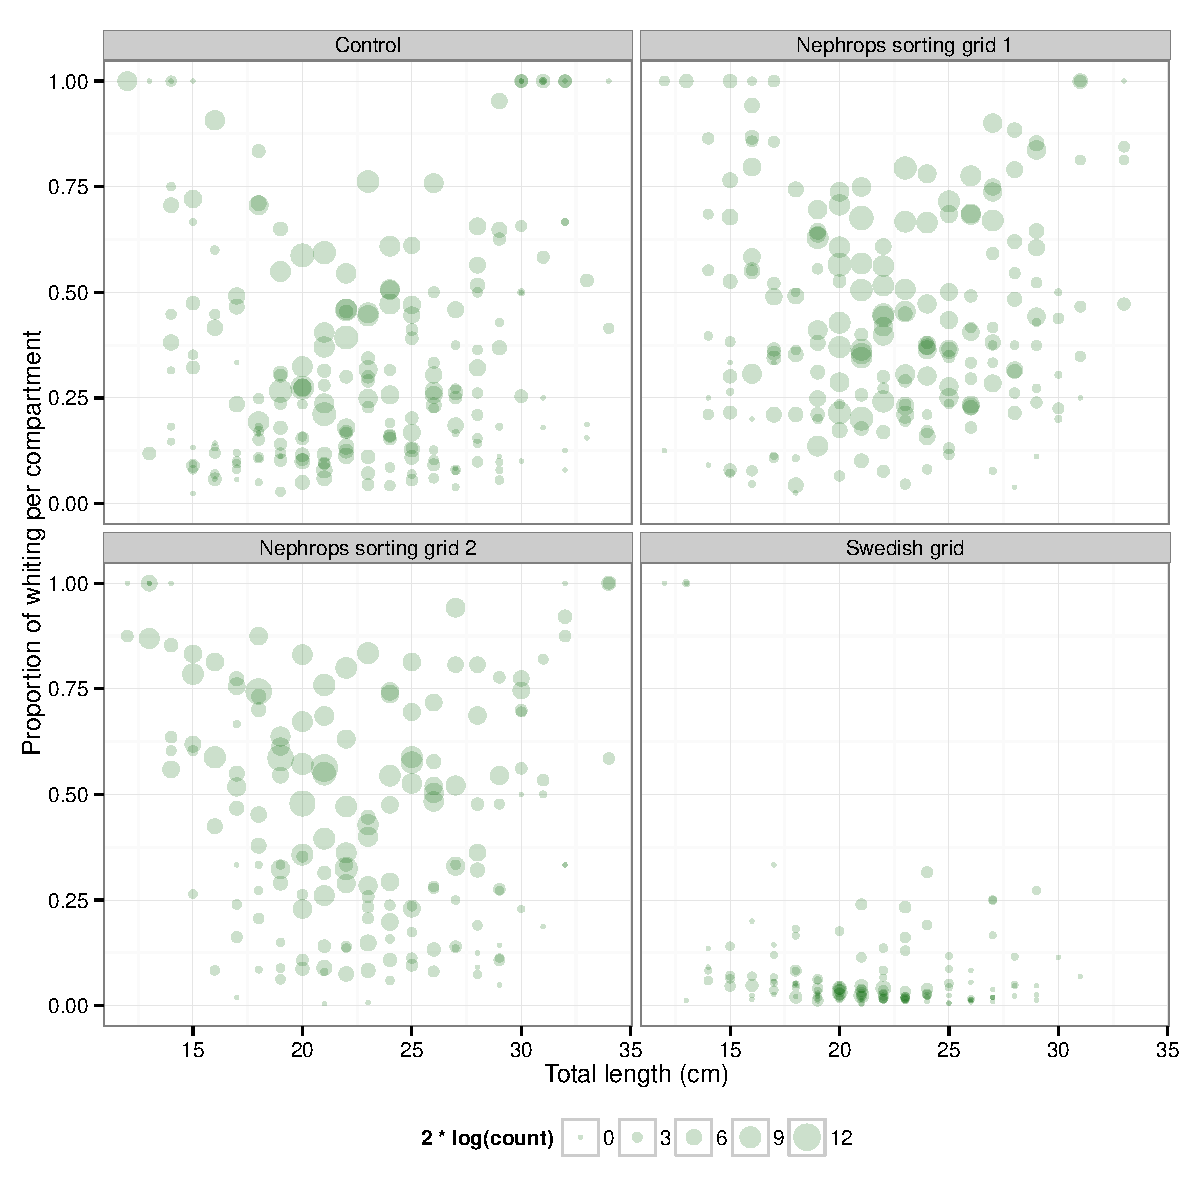
\includegraphics[width=\maxwidth]{figure/unnamed-chunk-5-1} \caption[Proportion of whiting catch retained per haul]{Proportion of whiting catch retained per haul. Each point represents the proportion of raised whiting catch per haul and length class retained in a given cod-end (Control: CTRL, Nephrops sorting grid 1: NSG1, Nephrops sorting grid 2: NSG2, or the Swedish Grid). The size of the point is proportional to the log of the count.}\label{fig:unnamed-chunk-5}
\end{figure}


\end{knitrout}

\section{Model}
The first model we can use is a multinomial for the proportion retained in the four compartments. 

\begin{knitrout}\footnotesize
\definecolor{shadecolor}{rgb}{0.969, 0.969, 0.969}\color{fgcolor}\begin{kframe}
\begin{alltt}
\hlkwd{library}\hlstd{(nnet)}

\hlcom{## First fit is constant proportions}
\hlcom{## not accounting for length}

\hlstd{mnom0} \hlkwb{<-} \hlkwd{multinom}\hlstd{(whg.count.mat} \hlopt{~} \hlnum{1} \hlopt{+} \hlkwd{offset}\hlstd{(offset.mat))}
\end{alltt}
\begin{verbatim}
## # weights:  24 (3 variable)
## initial  value 6484.787263 
## final  value 5402.678685 
## converged
\end{verbatim}
\begin{alltt}
\hlcom{## second fit include net configuration/rotations}
\hlstd{mnom0.1} \hlkwb{<-} \hlkwd{multinom}\hlstd{(whg.count.mat} \hlopt{~} \hlstd{netconfig} \hlopt{+}
                    \hlkwd{offset}\hlstd{(offset.mat),} \hlkwc{data} \hlstd{= grid.whg.cast)}
\end{alltt}
\begin{verbatim}
## # weights:  36 (12 variable)
## initial  value 6484.787263 
## iter  10 value 4974.370768
## final  value 4833.915629 
## converged
\end{verbatim}
\begin{alltt}
\hlcom{## include carapace length polynomials of different complexity}
\hlstd{mnom1} \hlkwb{<-} \hlkwd{update}\hlstd{(mnom0.1, .} \hlopt{~} \hlstd{.} \hlopt{+} \hlkwd{poly}\hlstd{(TOTAL.LENGTH,} \hlnum{1}\hlstd{),}
                \hlkwc{data} \hlstd{= grid.whg.cast)}
\end{alltt}
\begin{verbatim}
## # weights:  40 (15 variable)
## initial  value 6484.787263 
## iter  10 value 4972.140159
## iter  20 value 4822.312835
## final  value 4822.310892 
## converged
\end{verbatim}
\begin{alltt}
\hlstd{mnom2} \hlkwb{<-} \hlkwd{update}\hlstd{(mnom0.1, .} \hlopt{~} \hlstd{.} \hlopt{+} \hlkwd{poly}\hlstd{(TOTAL.LENGTH,} \hlnum{2}\hlstd{),}
                \hlkwc{data} \hlstd{= grid.whg.cast)}
\end{alltt}
\begin{verbatim}
## # weights:  44 (18 variable)
## initial  value 6484.787263 
## iter  10 value 4967.527498
## iter  20 value 4820.324322
## final  value 4820.314123 
## converged
\end{verbatim}
\begin{alltt}
\hlstd{mnom3} \hlkwb{<-} \hlkwd{update}\hlstd{(mnom0.1, .} \hlopt{~} \hlstd{.} \hlopt{+} \hlkwd{poly}\hlstd{(TOTAL.LENGTH,} \hlnum{3}\hlstd{),} \hlkwc{data} \hlstd{= grid.whg.cast)}
\end{alltt}
\begin{verbatim}
## # weights:  48 (21 variable)
## initial  value 6484.787263 
## iter  10 value 4966.280119
## iter  20 value 4820.170772
## final  value 4819.869672 
## converged
\end{verbatim}
\begin{alltt}
\hlstd{mnom4} \hlkwb{<-} \hlkwd{update}\hlstd{(mnom0.1, .} \hlopt{~} \hlstd{.} \hlopt{+} \hlkwd{poly}\hlstd{(TOTAL.LENGTH,} \hlnum{4}\hlstd{),} \hlkwc{data} \hlstd{= grid.whg.cast)}
\end{alltt}
\begin{verbatim}
## # weights:  52 (24 variable)
## initial  value 6484.787263 
## iter  10 value 4964.317977
## iter  20 value 4814.728213
## iter  30 value 4814.192615
## iter  30 value 4814.192596
## iter  30 value 4814.192596
## final  value 4814.192596 
## converged
\end{verbatim}
\begin{alltt}
\hlkwd{AIC}\hlstd{(mnom0, mnom0.1, mnom1, mnom2, mnom3, mnom4)}
\end{alltt}
\begin{verbatim}
##         df       AIC
## mnom0    3 10811.357
## mnom0.1 12  9691.831
## mnom1   15  9674.622
## mnom2   18  9676.628
## mnom3   21  9681.739
## mnom4   24  9676.385
\end{verbatim}
\begin{alltt}
\hlcom{## looks like a quadratic carapace length effect fits best}
\end{alltt}
\end{kframe}
\end{knitrout}


Get predictions for the fitted model (note that this is run in a cleaner fashion in the ADMB fit below).

\begin{knitrout}\footnotesize
\definecolor{shadecolor}{rgb}{0.969, 0.969, 0.969}\color{fgcolor}\begin{kframe}
\begin{alltt}
\hlcom{## get predictions manually}
\hlcom{## CIs not defined in multinomial context but let's try}

\hlstd{best.model} \hlkwb{<-} \hlstd{mnom2}

\hlcom{## fit coefficients}
\hlstd{beta.mu} \hlkwb{<-} \hlkwd{c}\hlstd{(}\hlkwd{t}\hlstd{(}\hlkwd{coef}\hlstd{(best.model)))}

\hlcom{## fit coefficient variance covariance matrix}
\hlstd{Sigma} \hlkwb{<-} \hlkwd{vcov}\hlstd{(best.model)}

\hlcom{## number of lengths to predict for}
\hlstd{nlength} \hlkwb{<-} \hlnum{50}

\hlstd{pred.length} \hlkwb{<-} \hlkwd{seq}\hlstd{(}\hlkwd{min}\hlstd{(grid.whg.cast}\hlopt{$}\hlstd{TOTAL.LENGTH),}
                   \hlkwd{max}\hlstd{(grid.whg.cast}\hlopt{$}\hlstd{TOTAL.LENGTH),} \hlkwc{length} \hlstd{= nlength)}

\hlcom{## get the polynomial of lengths}
\hlstd{polyfun} \hlkwb{<-} \hlkwd{poly}\hlstd{(grid.whg.cast}\hlopt{$}\hlstd{TOTAL.LENGTH,} \hlnum{2}\hlstd{)}

\hlcom{## model matrix}
\hlstd{Xpred} \hlkwb{<-} \hlkwd{cbind}\hlstd{(}\hlnum{1}\hlstd{,} \hlnum{1}\hlopt{/}\hlnum{3}\hlstd{,} \hlnum{1}\hlopt{/}\hlnum{3}\hlstd{,} \hlnum{1}\hlopt{/}\hlnum{3}\hlstd{,} \hlkwd{predict}\hlstd{(polyfun, pred.length))}

\hlcom{## number of times to resample predictions to get CIs}
\hlstd{nresamp} \hlkwb{<-} \hlnum{1e3}
\hlstd{pred.array} \hlkwb{<-} \hlkwd{array}\hlstd{(}\hlnum{NA}\hlstd{,} \hlkwc{dim} \hlstd{=} \hlkwd{c}\hlstd{(nlength,} \hlnum{4}\hlstd{, nresamp))}

\hlcom{## package to draw from multivariate normal }
\hlkwd{library}\hlstd{(mvtnorm)}

\hlkwa{for}\hlstd{(i} \hlkwa{in} \hlnum{1}\hlopt{:}\hlstd{nresamp)\{}
  \hlcom{##print(i)}
  \hlstd{beta0} \hlkwb{<-} \hlkwd{matrix}\hlstd{(}\hlkwd{rmvnorm}\hlstd{(}\hlnum{1}\hlstd{,} \hlkwc{mean} \hlstd{= beta.mu,} \hlkwc{sigma} \hlstd{= Sigma),}
                  \hlkwc{nrow} \hlstd{=} \hlnum{3}\hlstd{,} \hlkwc{byrow} \hlstd{=} \hlnum{TRUE}\hlstd{)}
  \hlstd{beta} \hlkwb{<-} \hlkwd{cbind}\hlstd{(}\hlnum{0}\hlstd{,} \hlkwd{t}\hlstd{(beta0))}
  \hlstd{eta} \hlkwb{<-} \hlstd{Xpred} \hlopt \hlstd{beta}
  \hlstd{pred.p} \hlkwb{<-} \hlkwd{exp}\hlstd{(eta)} \hlopt{/} \hlkwd{rowSums}\hlstd{(}\hlkwd{exp}\hlstd{(eta))}
  \hlstd{pred.array[ , , i]} \hlkwb{<-} \hlstd{pred.p}
  \hlkwd{rm}\hlstd{(pred.p)}
\hlstd{\}}

\hlcom{## mean across samples}
\hlstd{pred.mu} \hlkwb{<-} \hlkwd{apply}\hlstd{(pred.array,} \hlkwd{c}\hlstd{(}\hlnum{1}\hlstd{,} \hlnum{2}\hlstd{), mean)}

\hlcom{## upper across samples}
\hlstd{pred.upper} \hlkwb{<-} \hlkwd{apply}\hlstd{(pred.array,} \hlkwd{c}\hlstd{(}\hlnum{1}\hlstd{,} \hlnum{2}\hlstd{), quantile,} \hlkwc{p} \hlstd{=} \hlnum{0.975}\hlstd{)}

\hlcom{## lower across samples}
\hlstd{pred.lower} \hlkwb{<-} \hlkwd{apply}\hlstd{(pred.array,} \hlkwd{c}\hlstd{(}\hlnum{1}\hlstd{,} \hlnum{2}\hlstd{), quantile,} \hlkwc{p} \hlstd{=} \hlnum{0.025}\hlstd{)}

\hlcom{## bring all together in a data frame for ggplot}
\hlstd{m} \hlkwb{<-} \hlkwd{dim}\hlstd{(pred.mu)[}\hlnum{1}\hlstd{]}

\hlstd{pred.ci.df} \hlkwb{<-} \hlkwd{data.frame}\hlstd{(}
                \hlkwc{COMPARTMENT} \hlstd{=} \hlkwd{rep}\hlstd{(}\hlkwd{c}\hlstd{(}\hlstr{"Control"}\hlstd{,} \hlstr{"Nephrops sorting grid 1"}\hlstd{,}
                  \hlstr{"Nephrops sorting grid 2"}\hlstd{,} \hlstr{"Swedish grid"}\hlstd{),} \hlkwc{each} \hlstd{= m),}
                \hlkwc{TOTAL.LENGTH} \hlstd{=} \hlkwd{rep}\hlstd{(pred.length,} \hlkwc{times} \hlstd{=} \hlnum{4}\hlstd{),}
                \hlkwc{proportion} \hlstd{=} \hlkwd{c}\hlstd{(pred.mu),}
                \hlkwc{lower} \hlstd{=} \hlkwd{c}\hlstd{(pred.lower),}
                \hlkwc{upper} \hlstd{=} \hlkwd{c}\hlstd{(pred.upper))}
\end{alltt}
\end{kframe}
\end{knitrout}

Finally overlay the fit on the sample proportions

\begin{knitrout}\footnotesize
\definecolor{shadecolor}{rgb}{0.969, 0.969, 0.969}\color{fgcolor}\begin{kframe}
\begin{alltt}
\hlstd{p} \hlopt{+} \hlkwd{geom_ribbon}\hlstd{(}\hlkwc{data} \hlstd{= pred.ci.df,} \hlkwd{aes}\hlstd{(}\hlkwc{ymin} \hlstd{= lower,} \hlkwc{ymax} \hlstd{= upper),}
                \hlkwc{alpha} \hlstd{=} \hlnum{0.3}\hlstd{,} \hlkwc{fill} \hlstd{=} \hlstr{"purple"}\hlstd{)} \hlopt{+}
  \hlkwd{geom_line}\hlstd{(}\hlkwc{data} \hlstd{= pred.ci.df,} \hlkwd{aes}\hlstd{(}\hlkwc{x} \hlstd{= TOTAL.LENGTH,} \hlkwc{y} \hlstd{= proportion),}
            \hlkwc{col} \hlstd{=} \hlstr{"purple"}\hlstd{,} \hlkwc{size} \hlstd{=} \hlnum{0.5}\hlstd{)} \hlopt{+}
  \hlkwd{geom_hline}\hlstd{(}\hlkwd{aes}\hlstd{(}\hlkwc{yintercept} \hlstd{=} \hlnum{0.25}\hlstd{),} \hlkwc{linetype} \hlstd{=} \hlstr{"dashed"}\hlstd{)}
\end{alltt}
\end{kframe}\begin{figure}
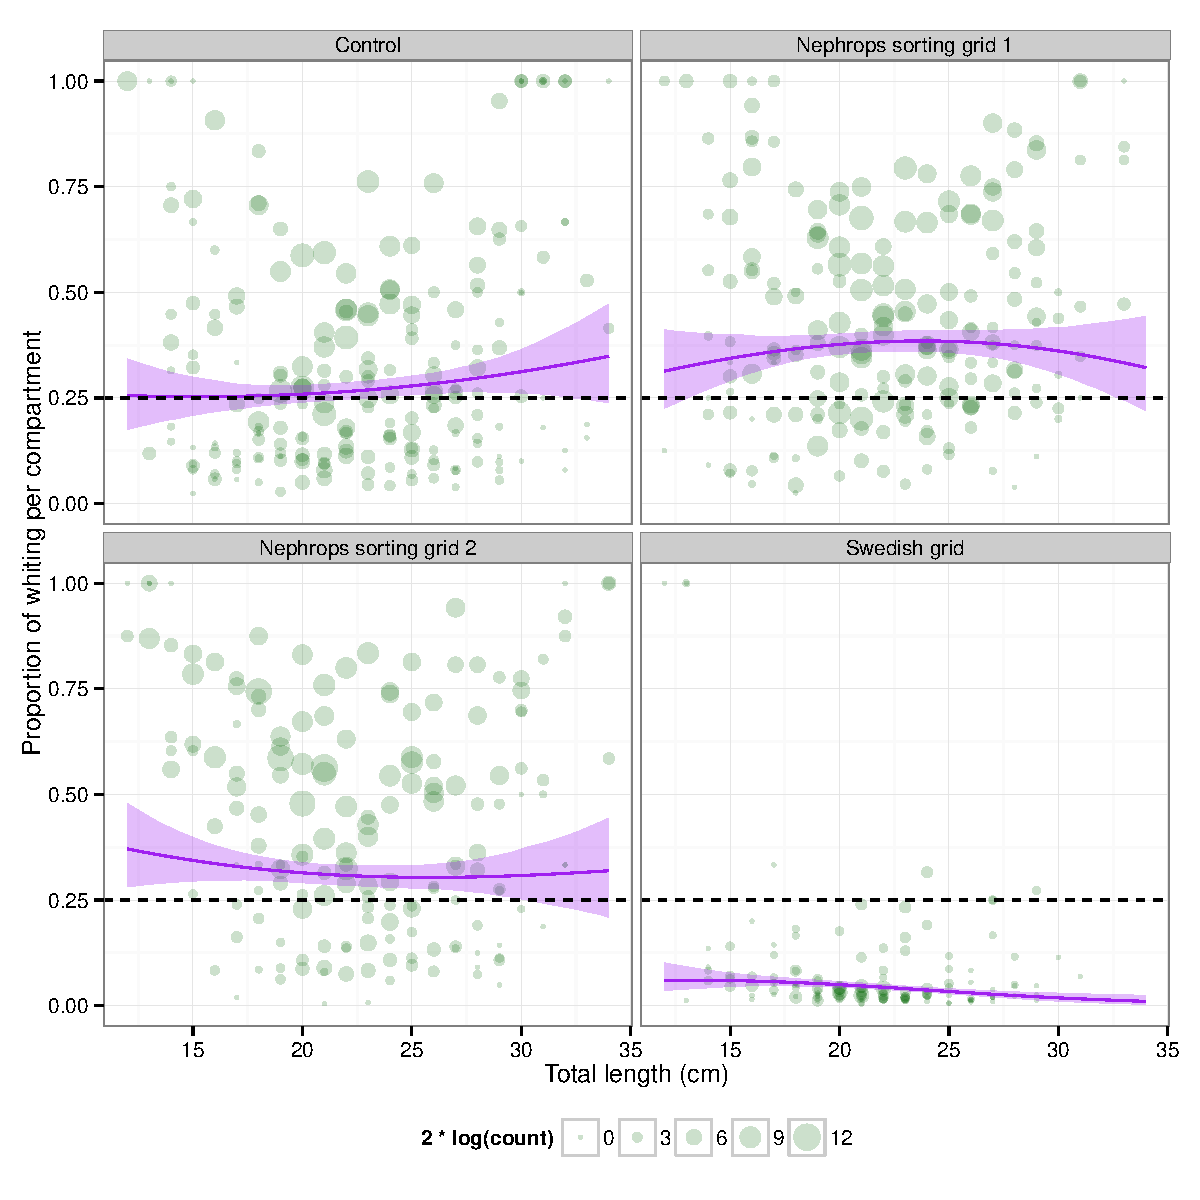
\includegraphics[width=\maxwidth]{figure/unnamed-chunk-8-1} \caption[Proportion of whiting catch retained per haul with fitted multinomial model (without a weight effect or random effects) and associated re-sampled intervals]{Proportion of whiting catch retained per haul with fitted multinomial model (without a weight effect or random effects) and associated re-sampled intervals. Null hypothesis of equal retention is displayed as the dashed line at 0.25.}\label{fig:unnamed-chunk-8}
\end{figure}


\end{knitrout}

Overlay the model predictions

\begin{knitrout}\footnotesize
\definecolor{shadecolor}{rgb}{0.969, 0.969, 0.969}\color{fgcolor}\begin{kframe}
\begin{alltt}
\hlkwd{ggplot}\hlstd{(pred.ci.df,} \hlkwd{aes}\hlstd{(}\hlkwc{x} \hlstd{= TOTAL.LENGTH,} \hlkwc{y} \hlstd{= proportion,} \hlkwc{group} \hlstd{= COMPARTMENT))} \hlopt{+} \hlkwd{geom_line}\hlstd{(}\hlkwd{aes}\hlstd{(}\hlkwc{colour} \hlstd{= COMPARTMENT))}  \hlopt{+} \hlkwd{theme}\hlstd{(}\hlkwc{legend.position} \hlstd{=} \hlstr{"bottom"}\hlstd{)} \hlopt{+} \hlkwd{geom_ribbon}\hlstd{(}\hlkwd{aes}\hlstd{(}\hlkwc{ymin} \hlstd{= lower,} \hlkwc{ymax} \hlstd{= upper,} \hlkwc{fill} \hlstd{= COMPARTMENT),} \hlkwc{alpha} \hlstd{=} \hlnum{0.3}\hlstd{)} \hlopt{+} \hlkwd{geom_hline}\hlstd{(}\hlkwc{yintercept} \hlstd{=} \hlnum{0.25}\hlstd{,} \hlkwc{linetype} \hlstd{=} \hlstr{"dashed"}\hlstd{)}
\end{alltt}
\end{kframe}\begin{figure}
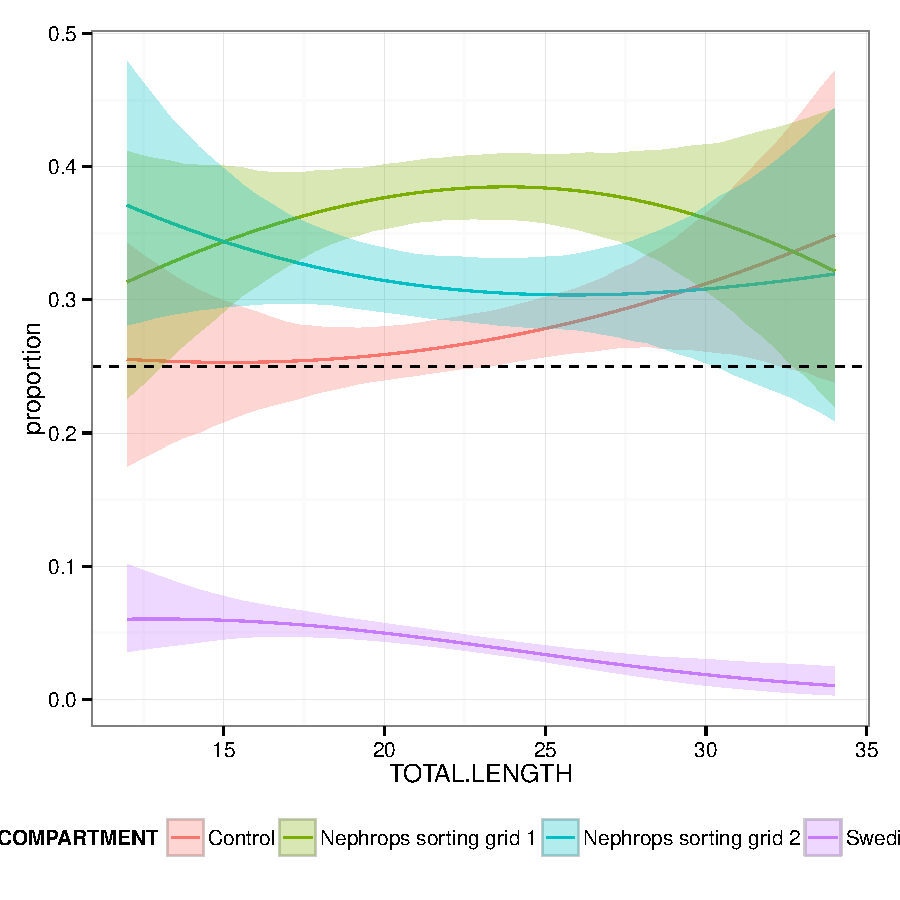
\includegraphics[width=\maxwidth]{figure/unnamed-chunk-9-1} \caption[ Multinomial model predicted proportion of whiting catch retained by compartment]{ Multinomial model predicted proportion of whiting catch retained by compartment. No weight effects or random effects are incuded in this model. Null hypothesis of equal retention is displayed as the dashed line at 0.25.}\label{fig:unnamed-chunk-9}
\end{figure}


\end{knitrout}


\bibliography{../../../../misc/epif_bibliography}
\bibliographystyle{../../../../misc/cjfas}
\end{document}

